\documentclass[conference]{IEEEtran}
\usepackage{multirow}
\usepackage{subfigure}
\usepackage{graphicx}
\usepackage{graphics}
\usepackage{rotating}
\usepackage{verbatim}
\usepackage{float}
\usepackage{url}
\restylefloat{table}
\ifCLASSINFOpdf
\else
\fi
\hyphenation{op-tical net-works semi-conduc-tor}
\begin{document}
\title{Dirt Spot Sweeping Random Strategy}
\author{\IEEEauthorblockN{Mian Asbat Ahmad}
\IEEEauthorblockA{Department of Computer Science\\
University of York\\
York, United Kingdom\\
Email: mian.ahmad@york.ac.uk}

\and
\IEEEauthorblockN{Manuel Oriol}
\IEEEauthorblockA{ABB Corporate Research\\
Industrial Software Systems\\
Baden-Dattwil, Switzerland\\
Email: manuel.oriol@ch.abb.com}}

\maketitle

%%%%%%%%%%%%%%%%%    ABSTRACT   %%%%%%%%%%%%%%%%%%%%
\begin{abstract}
While random testing has recently gained momentum, very little has been known on failure domains and their shape. 
This paper presents an enhanced and improved form of automated random testing, called the Dirt Spot Sweeping Random (DSSR) strategy. DSSR is a new strategy that takes the assumption that a number of failure domains are contiguous.
DSSR starts as a regular random+ testing session --- a random testing session with some preference for boundary values. 
When a failure is found, it increases the chances of using neighbouring values in subsequent tests, thus slowly sweeping around the failure found in hope of finding failures from a different kind in its vicinity.

DSSR was implemented within the YETI random testing tool. We evaluate DSSR against random+ and pure random strategies by testing 80 classes with $10^5$ calls for each session 30 times for each strategy.
Our findings are that in 68\% of the cases all three strategies all find the same faults, in 10\% of cases random+ perfroms better, in 12\% pure random performs better, and 10\% DSSR performed better.
Overall, DSSR also found 5\% more failures than other strategies.
\end{abstract}
\IEEEpeerreviewmaketitle

%Several (enhanced/new/efficient) random strategies are based on the presence of point, block and strip patterns across the input domain. Emphasis of each one is to select test input farthest away from each other to increase the chances of targeting these faulty patterns to produce better results than pure random strategy. However no strategy has tried to expose these contiguous fault pattern once they are discovered during testing. 
%
%In this paper, we propose DSSR, a new random strategy that discovers contiguous faults  and evaluate it against Random and pure random. Results show that DSSR is better in some cases and random+ in most other cases. Because all strategies have the same potential, they exhibit similar numbers, but none of them is fundamentally better than the others.



%%%%%%%%%%%%%%%%%    INTRODUCTION   %%%%%%%%%%%%%%%%%%%%
\section{Introduction}\label{sec:intro}
Success of a software testing technique is mainly based on the number of faults it discovers in the Software Under Test (SUT). An efficient testing process discovers the maximum number of faults in a minimum possible amount of time. Exhaustive testing where software is tested against all possible inputs is, in most cases, not feasible because of the size of the input domain, limited resources and strict time constraints. Therefore, strategies in automated software testing tools are developed with the aim to select more fault-finding test input from the input domain for the given SUT. Producing such targeted test input is difficult because each system has its own requirements and functionality.

Chan et al.~\cite{Chan1996} discovered that there are patterns of failure causing inputs across the input domain. They divided the patterns into point, block and strip patterns on the basis of their occurrence across the input domain. In another study, Chen et al.~\cite{Chen2008} found that the performance of random testing can be increased by slightly altering the technique of test case selection. In adaptive random testing, they found that the performance of random testing increases by up to 50\% when test input is selected evenly across the whole input domain. This was mainly attributed to the better distribution of input which increased the chance of selecting inputs from failure patterns. Similarly Restricted Random Testing \cite{Chan2002}, Feedback directed Random Test Generation \cite{Pacheco2007a}, Mirror Adaptive Random Testing \cite{Chen2003} and Quasi Random Testing \cite{Chen2005} also stress on the need of test case selection covering the whole input domain to improve results.

In this paper we take the assumption that in a significant number of classes failure domains are contiguous or are very close by. From this assumption, we devised the Dirt Spot Sweeping\footnote{The name refers to the cleaning robots strategy to insist on places where dirt has been found in large amount.} Random strategy (DSSR) which starts as a random+ strategy --- random strategy focusing more on boundary values. When it finds a new failure, it then increases the chances of testing using neighbouring values. Of course, since this strategy is also a random testing strategy, it has the potential to find all failures in the program, but we expect it to be faster at finding unique failures for classes in which failure domains are contiguous than the pure random (R) and random+ (R+) strategies.

We implemented DSSR as a strategy for the random testing tool YETI\footnote{\url{http://www.yetitest.org}}. To evaluate our approach, we tested thirty times each one of 80 classes from the Qualitas Corpus\footnote{\url{http://www.qualitascorpus.com}} with each of the three strategies DSSR, R, and R+. We found that in 68\% of the cases all three strategies all find the same faults, in 10\% of cases random+ perfroms better, in 12\% pure random performs better, and 10\% DSSR performed better.
Overall, DSSR also found 5\% more failures than other strategies.

%//MANUEL: WHAT IS THIS??
%Motivated by research work underlying Proportional Sampling Strategy of the patterns of failure causing inputs across the input domain, we thought an enhanced random testing technique called Dirt Spot Sweeping Random (DSSR) strategy. The main emphasis in DSSR strategy is focused on the patterns of failures for better performance. Experiments were conducted to address the following research issues:
%\begin{enumerate}
%
%\item To get highly efficient algorithm for coping with the combination of strategies including pure random, random plus and spot sweeping.
%
%\item To get high number of unique faults in the SUT. 
%
%\item To get lower number of unique faults and higher number of similar faults in the SUT.
%
%\item  To examine no/negative improvement in test results of the SUT. 
%
%\item  To determine the processing time involved in DSSR strategy.
%
%\end{enumerate}
The rest of this paper is organized as follows: \\
Section~\ref{sec:dssr} describes the DSSR strategy. Section~\ref{sec:imp} presents our implementation of the strategy. Section~\ref{sec:eval} explains our experimental setup. Section~\ref{sec:res} shows the results of our experiments. Section~\ref{sec:discussion} discusses the results. Section~\ref{sec:rw} presents related work and we conclude in Section~\ref{sec:conc}.




%%%%%%%%%%%%%%%%%    DIRT SPOT SWEEPING STRATEGY  %%%%%%%%%%%%%%%

\section{Dirt Spot Sweeping Random Strategy}\label{sec:dssr}
The Dirt Spot Sweeping Random (DSSR) strategy is a new strategy which combines the random+ strategy and with a dirt spot sweeping dunctionality. The strategy is based on two intuitions. One is that boundaries have interesting values and using these values in isolation can provide high impact on test results, the other is that faults reside in contiguous blocks and stripes. If this is the case, DSSR increases the performance of the test strategy in terms of executing fewer numbers of test cases with higher number of faults. Each strategy is briefly explained as follows.

\subsection{Random (R)}
The pure random strategy is a black-box testing technique in which the SUT is executed using randomly selected test data. Test results obtained are compared to the defined oracle, using SUT specifications in the form of contracts or assertions. In the absence of contracts and assertions the exceptions defined by the programming language are used as test oracle. 
%According to Beizer \cite{Beizer1990}, software performance is directly dependent on the combination of two main factors, correctness and robustness. Correctness is the expected behaviour of the software based on its specifications while robustness is the behaviour of the software that is not defined in its specifications. 
%Since random testing generates test data randomly, without any specific pattern, it effectively tests the performance of software by evaluating it for both correctness and robustness. 
Because of its black-box testing nature, this strategy is particularly effective in testing softwares where the developers want to keep the source code secret~\cite{Chen2010}. The generation of random test data is comparatively cheap and does not require too much intellectual and computation efforts~\cite{Ciupa2009, Ciupa2008}. It is mainly for this reason that various researchers have recommended this strategy for incorporation in automatic testing tools \cite{Ciupa2008a}. YETI \cite{Oriol2010a}, \cite{Oriol2010}, AutoTest \cite{Leitner2007}, \cite{Ciupa2007}, QuickCheck \cite{Claessen2000}, Randoop \cite{Pacheco2007}, Jartage \cite{Oriat2004} are some of the most common automated testing tools based on random strategy.\\
\indent Efficiency of random testing was made suspicious with the intuitive statement of Myers \cite{Myers2004} who termed random testing as one of the poorest methods for software testing. however, experiments performed by various researchers, \cite{Ciupa2007}, \cite{Duran1981}, \cite{Duran1984}, \cite{Hamlet1994} and \cite{Ntafos2001} have experimentally proved that random testing is simple to implement, cost effective, highly efficient and free from human bias as compared to its rival techniques.\

Because programs tested at random typically fail a large number of times (there are a large number of calls), it is necessary to cluster failures that likely represent the same fault. The traditional way of doing it is to compare the full stack traces and error types and use this as an equivalence class~\cite{Ciupa2007,Oriol2012} called a unique failures. This way of grouping failures is also used in random+ and DSSR.


\subsection{Random Plus Strategy (R+)}
The random+ strategy \cite{Leitner2007} is an extension of the pure random strategy. It uses some special pre-defined values which can be simple boundary values or values that have high tendency of finding faults in the SUT. Boundary values \cite{Beizer1990} are the values on the start and end of a particular type. For instance, such values for \verb+int+ could be \verb+MAX_INT+, \verb+MAX_INT-1+, \verb+MIN_INT+, \verb-MIN_INT+1-, \verb+-1+, \verb+0+, \verb+1+.


%For instance, if input for a SUT is days of an year which is expressed in numbers from 1 to 365 then -3, -2, -1, 0, 1, 2, 3, 362, 363, 364, 365, 366, 367, 368 can be considered as border values as shown in Figure \ref{fig:boundaryValues}. 
%
%\begin{figure}[ht]
%\centering
%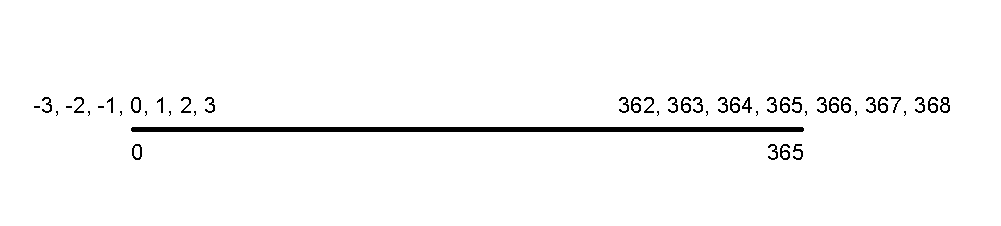
\includegraphics[width= 9cm,height=2cm]{boundary.png}
%\caption{Boundary values for input domain from 1 to 365}
%\label{fig:boundaryValues}
%\end{figure}

Similarly the tester might also add some other special values that he considers effective in finding faults for the current SUT. For example, if a program under test has a loop from -50 to 50 then the tester can add -55 to -45, -5 to 5, 45 to 55 etc. to the pre-defined list of special values in order to be selected for a test. This static list of interesting values is manually updated before the start of the test and has slightly high priority than selection of random values because of more relevance and high chances of finding faults for the given SUT. These special values have high impact on the results particularly detecting problems in specifications \cite{Ciupa2008}.


\subsection{Dirt Spot Sweeping}
Chan et al. \cite{Chan1996} found that there are patterns of failure-causing inputs across the input domain. Figure \ref{fig:patterns} shows these patterns for two dimensional input domain. They divided these patterns into three types called points, block and strip patterns. The black area (Points, block and strip) inside the box show the input which causes the system to fail while white area inside the box represent the genuine input. Boundary of the box (black solid line) surrounds the complete input domain and also represents the boundary values. They also argue that a strategy has more chances of hitting these fault patterns if test cases far away from each other are selected. Other researchers, \cite{Chan2002}, \cite{Chen2003} and \cite{Chen2005}, also tried to generate test cases further away from one another targeting these patterns and achieved higher performance.

\begin{figure}[ht]                                    
\centering
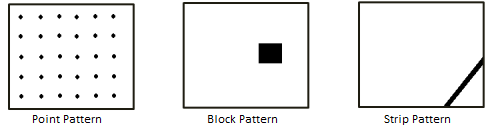
\includegraphics[width= 8cm,height=2.5cm]{ART_Patterns.png}
\caption{Failure patterns across input domain \cite{Chen2008}}
\label{fig:patterns}
\end{figure}

Spot sweeping is the part of DSSR strategy that comes into action when a a new unique failure is found in the system. On finding fault, it immediately adds the value causing the fault and its neighbouring values to the already existing list of interesting values. For example in a program if int type value 50 causes a fault in the system then spot sweeping will add values from 47 to 53 to the list of interesting values. Now if the fault lies in the block or strip pattern then adding its neighbours will explore all the unique failures present in that block or strip. As against random plus where the list of interesting values remain static, the list of interesting values is dynamic and changes during the test execution of each program in DSSR strategy.

\begin{figure}[ht]
\centering
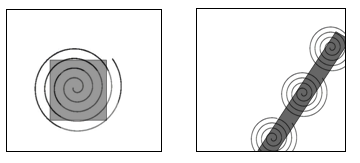
\includegraphics[width=8cm,height=2cm]{block2.png}
\caption{DSSR covering block and strip pattern}
\label{fig:block2}
\end{figure}

Figure \ref{fig:block2} shows how spot sweeping explores the faults residing in the block and strip patterns of a program. The faults coverage from the pattern is shown in spiral form because first fault will lead to second, second to third and so on till the end. In case the fault is positioned on the point pattern then the added values will not be very effective because point pattern is only an arbitrary fault point in the whole input domain.

\subsection{Structure of Dirt Spot Sweeping Random Strategy}

\hspace{10 mm}The DSSR strategy is explained with the help of flow-chart in Figure \ref{fig:Working_DSSS}. In this process the strategy continuously track the number of faults during the execution of the test session. To keep the system fast this tracking is done in a very effective way with zero or minimum overhead \cite{Leitner2009}. Execution of test is performed normally until a fault is found in the SUT. Then the program not only copy the value that lead to the fault, but also copy its surrounding values to the variable list of interesting values. It is evident from the flow-chart that if the fault finding value is of primitive type then the DSSR finds the type of the value and add values only of that particular type to the interesting values. Addition of these values increases the size of the list of interesting values that provide relevant test data for the remaining test session and the new generated test cases are more targeted towards finding new faults in the given SUT.\\
\begin{figure}[ht]
\centering
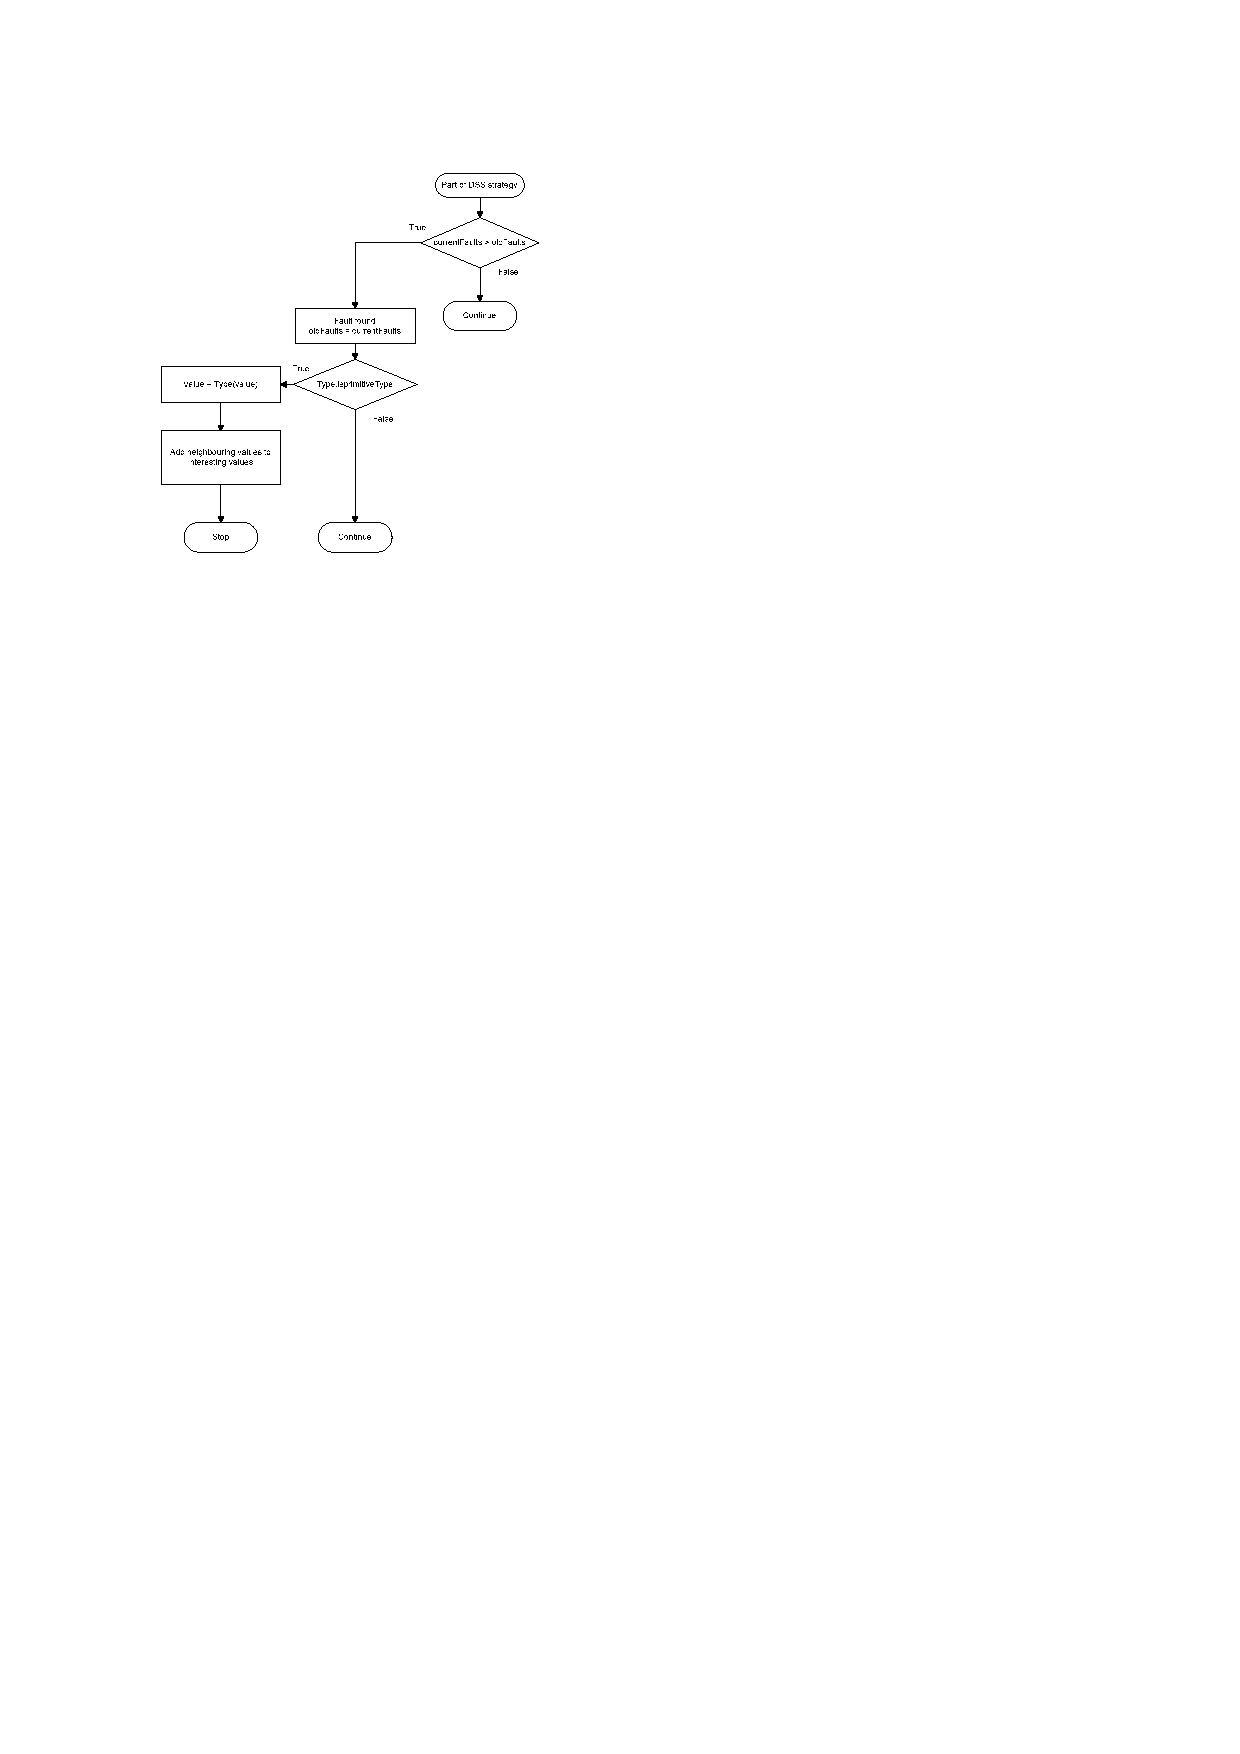
\includegraphics[width=8cm,height=9cm]{flowchart1.pdf}
\caption{Working mechanism of DSSR Strategy}
\label{fig:Working_DSSS}
\end{figure}

Border values and other special values that have high tendency of finding faults in the SUT are added to the list by random plus strategy prior to the start of test session where as to sweep the failure pattern, fault-finding value and its surrounding values are added at run time after a fault is found. Table \ref{table:addvalues} contain the values that are added to the list of interesting values when a fault is found. In the table test value is represented by X where X can be int, double, float, long, byte, short, char and String. All values are converted to their respective types before adding to the list of interesting values and vice versa.

\begin{table}[ht]
%\scriptsize
\caption{Neighbouring values for primitive types and String} % title of Table
\centering % used for centering table
\begin{tabular}{| l | l |} % centered columns (4 columns)
\hline\hline %inserts double horizontal lines
Type & Values to be added\\ [0.5ex] % inserts table
%heading
\hline % inserts single horizontal line
\multirow{1}{*}{X is int, double, float, } & ~ X,  X+1, X+2, X-1, X-2 \\ % inserting body of the
\multirow{1}{*}{long, byte, short \& char} &  \\ 

\hline
\multirow{8}{*}{X is String} & ~ X\\ % inserting body of the table

& ~ X + ``  "\\ % inserting body of the table
& ~ ``  " + X \\ % inserting body of the table
& ~ X.toUpperCase() \\
& ~ X.toLowerCase() \\
& ~ X.trim() \\
& ~ X.substring(2) \\
& ~ X.substring(1, X.length()-1) \\[1ex]
\hline
\hline %inserts single line
\end{tabular}
\label{table:addvalues} % is used to refer this table in the text
\end{table}





%%%%%%%%%%%%%%%%%%%%%%%%%%%%% EXPLANATION OF DSSR STRATEGY %%%%%%%%%%%%%%%%%%%%%%%%%%


\subsection{Explanation of DSSR with an example program}
The concept of DSSR strategy is explained through a simple program seeded with at least three faults. The first is division by zero exception denoted by 1 while the second and third are in the form of assertion statements denoted by 2 and 3 in the following program.  Below we describe how DSSR strategy perform execution when the following class is expose to testing.\\


\begingroup

    \fontsize{7pt}{8pt}\selectfont
    
\noindent
/\textasteriskcentered \textasteriskcentered \\*
\textasteriskcentered   ~ Calculate square of given number and verify results. \\*
\textasteriskcentered   ~ Code contain 3 faults.\\*
\textasteriskcentered   ~ @author (Mian and Manuel) \\* 
\textasteriskcentered   ~ @version (1.1, 11/07/12)\\*
\textasteriskcentered / \\*

\noindent public class Math1 \{\\
\indent public void calc (int num1) \{\\

\indent // Square num1 and store result.\\*
\indent int result1 = num1 * num1;\\*

%\indent \textbackslash\textbackslash Divide result1 by num1 and store result.\\*
\indent int result2 = result1 / num1;............................................................. Fault 1\\

%\indent \textbackslash\textbackslash To check that the revert of result is the received value.\\*
\indent assert Math.sqrt(result1) == num1;.................................................. Fault 2\\

%\indent \textbackslash\textbackslash To check that the value of result is positive.\\*
\indent assert result1 $>$= num1;................................................................... Fault 3\\
\indent \}  \\*
\noindent\}\\

\endgroup
In the above code one primitive variable of type ``int" is used, therefore, the input domain for DSSR strategy is from -2,147,483,648 to 2,147,483,647. The strategy further select some values like 0, Integer.MIN\_VALUE and Integer.MAX\_VALUE as interesting values which are prioritized for selection as test values. 
As the test starts, three faults are quickly discovered by DSSR strategy in the following order.\\
\indent \textbf{Fault 1:} The DSSR strategy might select value 0 for variable ``num1"  in the first test case because 0 is available in the list of interesting values and therefore its priority for selection is higher than other values. This will cause Java to generate division by zero exception because any integer divided by zero is infinity.\\*
\indent \textbf{Fault 2:} After catching the first fault, the strategy adds it and its surrounding values to the list of interesting values which includes 0, 1, 2, 3 and -1, -2, -3 in this case. In the second test case DSSR strategy may pick -3 as a test value and lead to the second fault where assertion (2) will fail because the square root of 9 will be +3 instead of input value -3.\\*
\indent \textbf{Fault 3:} After few tests DSSR strategy may select Integer.MAX\_VALUE for variable ``num1"  from the list of interesting values which will lead to the 3rd fault because result1 will not be able to store the square of Integer.MAX\_VALUE. Instead of the actual square value Java will assign a negative value (Java language rule) to variable result1 that will lead to the violation of next assertion (3).\\*
\indent The above execution process explains that the pre-defined values including border values, fault-finding values and the surrounding values lead us to the available faults quickly and in small number of tests as compared to Random and Random plus strategy. Random and Random plus takes longer to discover the second and third fault because they again start searching for new faults randomly although the remaining faults are very close to the first one. 



%%%%%%%%%%%%%%%%%    IMPLEMENTATION OF DSSR STRATEGY   %%%%%%%%%%%%


\section{Implementation of DSSR strategy}\label{sec:imp}
To avoid reinventing the wheel, an existing open-source automated random testing tool called YETI \cite{Oriol2011}, \cite{Oriol2012} is used for implementing the DSSR strategy. YETI is developed in Java and is capable of testing systems developed in procedural, functional and object-oriented languages. Its language-agnostic meta model enables it to test programs written in multiple languages including Java, C\#, JML and .Net. The core features of YETI includes easy extensibility for future growth, speed of up to one million calls per minute on java code, real time logging, real time GUI support, ability to test programs using multiple strategies and auto generation of test report at the end of the test session. A number of hitherto faults have successfully been found by YETI in various production softwares \cite{Oriol2012}, \cite{Oriol2012}. \\
\indent YETI can be divided into three main sections including core infrastructure, language-specific bindings and strategies. The core infrastructure represents routines, a group of types and a pool of specific type objects. The language specific bindings contain the code to make the call and process the results. The strategies section defines the procedure of how to select the modules (classes) from the project, how to select routines (methods) from these modules and how to generate values for the instances involved inside these routines. Most common strategies are random and random plus while DSSR strategy is also added to this section with the class name YetiDSSRStrategy. It is extension of YetiRandomStrategy, which in itself is extension of an abstract class YetiStrategy. The class hierarchy is shown in Figure \ref{fig:hierarchyofDSSR}.

\begin{figure}[h]
\centering
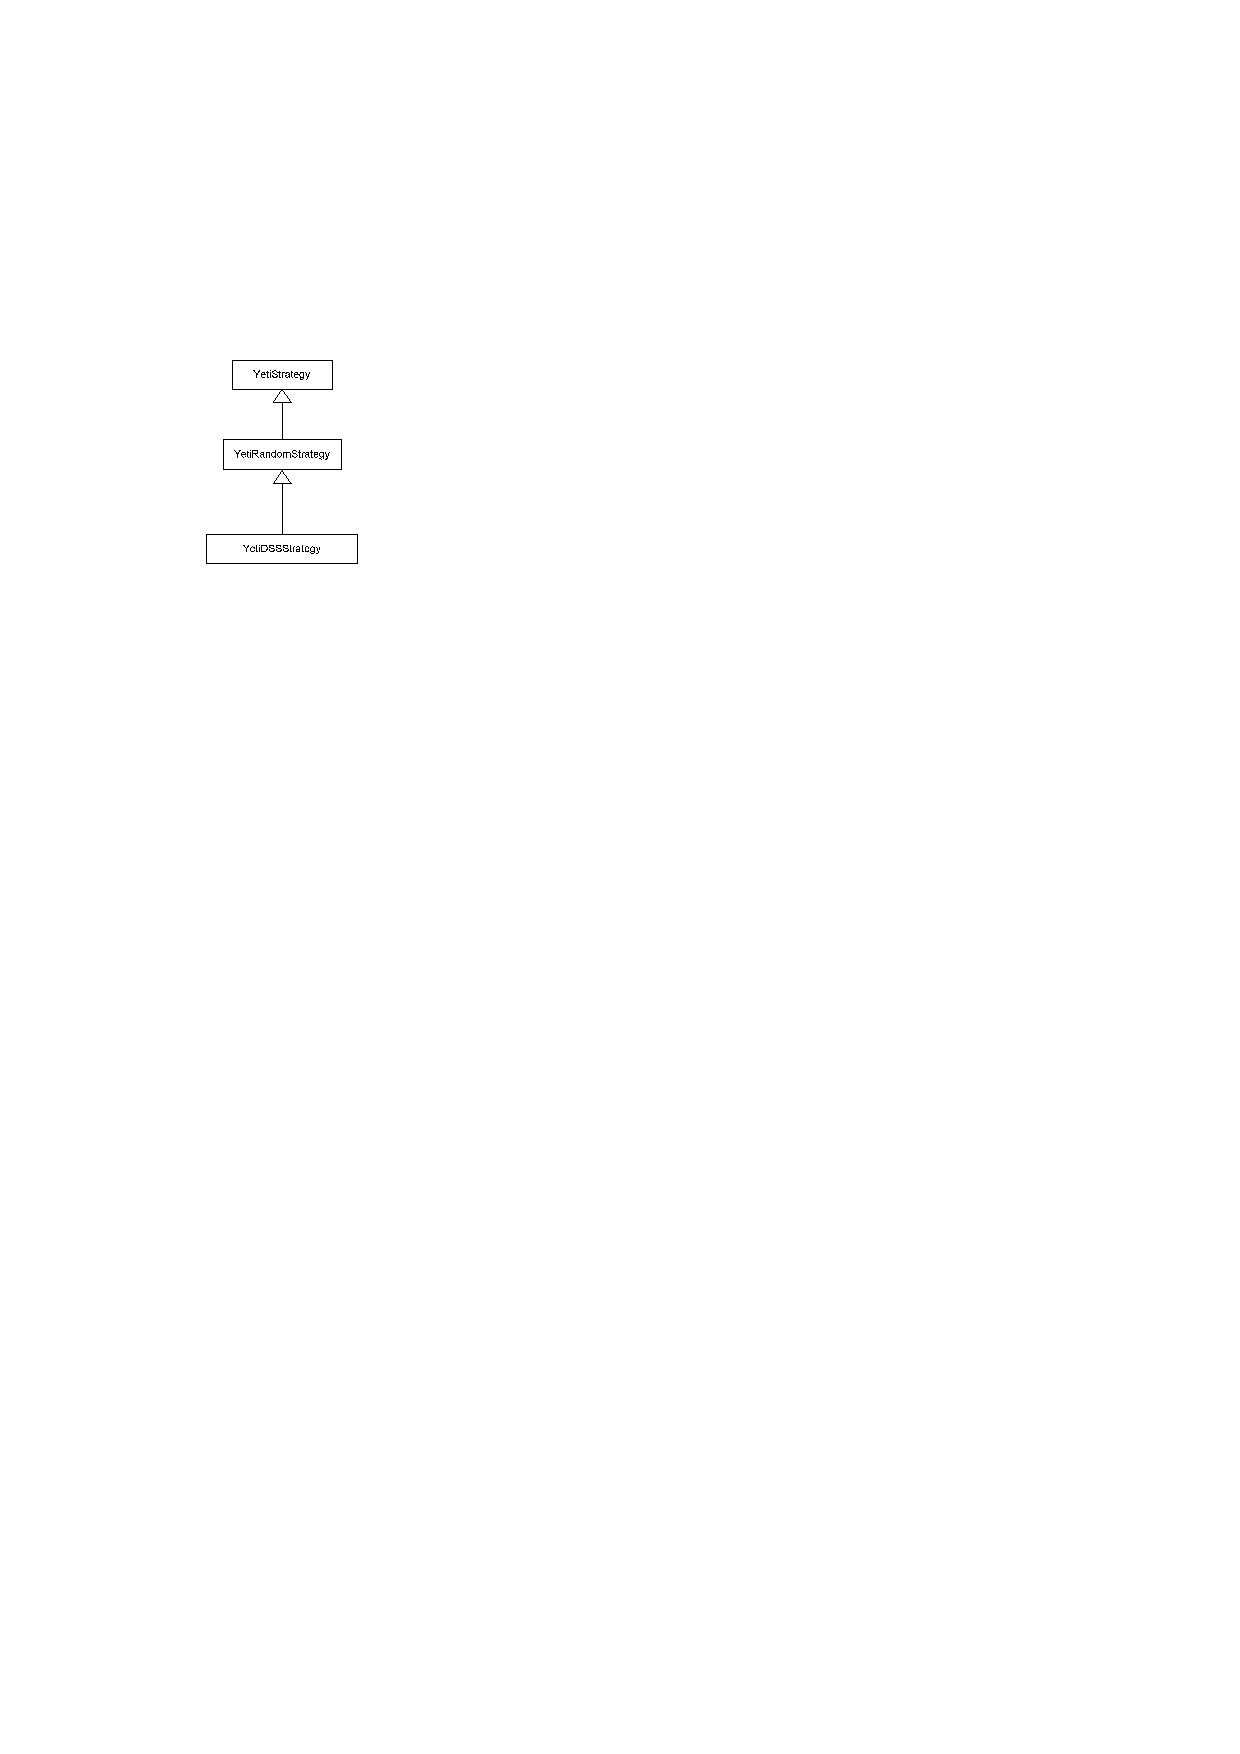
\includegraphics[width=4cm,height=4.5cm]{hierarchy.pdf}
\caption{Class Hierarchy of DSSR in YETI}
\label{fig:hierarchyofDSSR}
\end{figure}


By default YETI uses Random plus strategy if no particular strategy is defined during test initialization. It also enable the user to control the probability of null values and the percentage of newly created objects for each test session.\\
\indent YETI also provides an interactive Graphical User Interface (GUI) where user can see the progress of the current test in real time. Besides GUI, YETI also provides extensive logs of the test session, which are very helpful in fault tracking. For more details about YETI see references \cite{Oriol2010a} and \cite{Oriol2010}.

%%%%%%%%%%%%%%%%%    EVALUATION   %%%%%%%%%%%%%%%%%%%%


\section{Evaluation}\label{sec:eval}

To evaluate the DSSR strategy, we compare its performances to the performances of both pure random testing (R) and the random plus (R+)~\cite{Oriol2010} strategy. General factors such as system software and hardware as well as the YETI specific factors like percentage of null values, percentage of newly created objects and interesting value injection probability are kept constant for all the experiments.\\
\subsection{Experiments}

To evaluate the performances of the DSSR strategy we performed extensive testing of programs from the Qualitas Corpus \cite{Tempero2010a}. The Qualitas Corpus is a curated collection of open source java projects built with the aim of helping empirical research on  software engineering. These projects are collected in an organized form containing both the source and binary forms. The present evaluation uses version 20101126 which contains 106 open source java projects. We picked 80 classes at random from all classes in the Qualitas Corpus and test each of them thirty times with each strategy.
%It is available in two distributions. The release version ``r'' and the evolution version ``e''. The release version is compact size that contain only the recent version of the projects while the evolution version is more detailed which consists of more than 10 different versions of each project.\\
%Extensive experiments were carried out to evaluate the performance of DSSR strategy. Every class was tested 30 times by random, random plus and DSSR strategy. 
%The total number of testing sessions performed is 80 x 30 x 3 = 7200. 
Each class is evaluated through $10^5$ calls in each testing session.\footnote{The total number of tests is thus $80\times 30\times 3 \times 10^5 = 720\times 10^6~tests$.} 
Because of the absence of the contracts and assertions in the code under test, similarly to previous approaches~\cite{Oriol2012}, we use undeclared exceptions to compute unique failures found.

%\indent Commands for executing the experiments using pure random, random plus and DSSR strategies were as follows. Prog1 is the name of the class and nTests is the number of tests set to be executed during this experiment.\\
%
%\begingroup
%    \fontsize{7pt}{10pt}\selectfont
%\begin{itemize}
%\item java yeti.Yeti -java -testModules=Prog1 -nTests=10000 -nologs -gui -random.
%\item java yeti.Yeti -java -testModules=Prog1 -nTests=10000 -nologs -gui -randomPlus.
%\item java yeti.Yeti -java -testModules=Prog1 -nTests=10000 -nologs -gui -DSSR.\\
%\end{itemize}
%\endgroup
%
%

All tests are performed using a 64-bit Mac OS X Version 10.7.4 running on Intel(R) Core(TM)2 Duo CPU E8400 @ 3.00GHz with 6.00 GB RAM. Yeti runs on top of the Java(SE) Runtime Environment [Version 6.1.7601]. The machine took approximately 100 hours to process the experimental data.\\


%\subsection{Stability of experiments}
%Random strategies are characterized by using random input. In random strategy all the faults found in one test run may not necessarily be found in the second test run. Thus, the performance of random strategy cannot be evaluated with a few test sessions. To minimize the random behaviour of random testing every class was tested 30 times by each pure random, random plus and DSSR strategy. This was achieved by creating a batch executable script with the handy feature of YETI called Compact Report which logs each test report to a file for later evaluation.

\subsection{Performance measurement criteria}
Various measures including the E-measure, P-measure and F-measure have been used by researchers to find the effectiveness of the random test strategy. The E-measure (expected number of failures detected) and P-measure (probability of detecting at least one failure) were hevily criticized~\cite{Chen2008} and are not considered effective techniques for measuring efficiency of test strategy. The F-measure (number of test cases used to find the first fault) has been often used by researchers~\cite{Chen1996,Chen2004}. In our initial experiments the F-measure was used to evaluate the efficiency. Soon after a few experiments, it was realized that this was not the right choice because in some experiments the first strategy found first fault quickly than the second strategy but on the completion of test session the first strategy found lower number of total faults than the second strategy. Preference to a strategy only because it found the first fault better without giving due consideration to the total number of faults was not fair.

%%%%%%%%%% REMOVED as it is also present in future work. %%%%%%%%%%%%%%%%
\begin{comment}
Moreover, for random testing F-measure is quite unpredictable because its value can be easily increased by adding more narrow conditional statements in the SUT. For example in the following program it is difficult for random testing to generate the exact number (3.3338) quickly and therefore the F-measure will be high.\\*

\begingroup
    \fontsize{7pt}{8pt}\selectfont
\noindent
\{ \\*
\indent if ( (value $>$  3.3337) \&\& (value $<$ 3.3339) )\\*
\indent \{ 10/0 \} \\* 
\} \\*
\endgroup

\end{comment}
%%%%%%%%%%%%%%%%%%%%%%%%%%%%%
  
The literature review revealed that F-measure is used where testing stops after identification of first fault and the system is given back to the developers to remove the fault found. In such cases it make sense but now a days automated random testing tools test the whole system and print all of the faults found in one go therefore F-measure is not the favourable choice. Therefore in our experiments, performance of the strategy was measured in terms of finding maximum number of faults in a particular number of test calls   \cite{Pacheco2007a}, \cite{Ciupa2007}, \cite{Ciupa2008b}. This measurement was found effective because it clearly measured the performance of the strategy when all the other factors were kept constant.


%%%%%%%%%%%%%%%%%    RESULTS   %%%%%%%%%%%%%%%%%%%%

\section{Results}\label{sec:res}
Table \ref{table:Results} presents the results of 80 randomly selected classes evaluated by R, R+ and DSSR strategies. Table \ref{table:Results} figures contain name of the class (.class file), mean value, maximum number of faults, minimum number of faults and relative standard deviation for each of the 80 classes found by R, R+ and DSSR strategy. Total (table \ref{table:Results} last row) shows DSSR has higher mean value (1192.55) than R (1165.53) and R+ (1188.73). It also shows that DSSR found higher number of maximum faults (1234) and minimum faults (1126) than R (1181), (1055) and R+ (1224), (1127) respectively. The difference shows that DSSR found 10 (1234 - 1224 = 10 ) new faults that R+ couldn't discover while it found 53 (1234 - 1181= 53) new faults that R couldn't discover.\\
On analysis of the available data we found that results can be split up into six different categories as shown in figure \ref{fig:pie}. First category is the largest where each strategy performed equally well and found same number of faults after 1 lac tests. It contain 50 classes (62\% experiments) given in table \ref{table:equal}. Second category contain classes where R performed better than DSSR and R+. It contain 11 classes (14\% experiments) given in table \ref{fig:Randombetter}, figure \ref{fig:Randombetter}. Third category contain classes where R+ performed better than DSSR and R. It contain 7 classes (9\% experiments) given in table \ref{table:RandomPlusbetter}, figure \ref{fig:RandomPlusbetter}. Fourth Category contain classes where DSSR performed better than R and R+. It contain 7 classes (9\% experiments) given in table \ref{table:Randombetter}, figure \ref{fig:Randombetter}. Fifth Category contain only one class (1\%) where both DSSR and R found equal number of faults and performed better than R+ shown in table \ref{table:DSSRequaltoRandom}, figure \ref{fig:DSSRequaltoRandom} . Sixth Category contain classes where DSSR and R+ found equal number of faults and performed better than R. There are 4 classes (5\%) as shown in table \ref{table:DSSRequaltoRandomPlus}, figure \ref{fig:DSSRequaltoRandomPlus}. No class is found where R performs equal to R+.\\ 


\begin{figure}[ht]
\centering
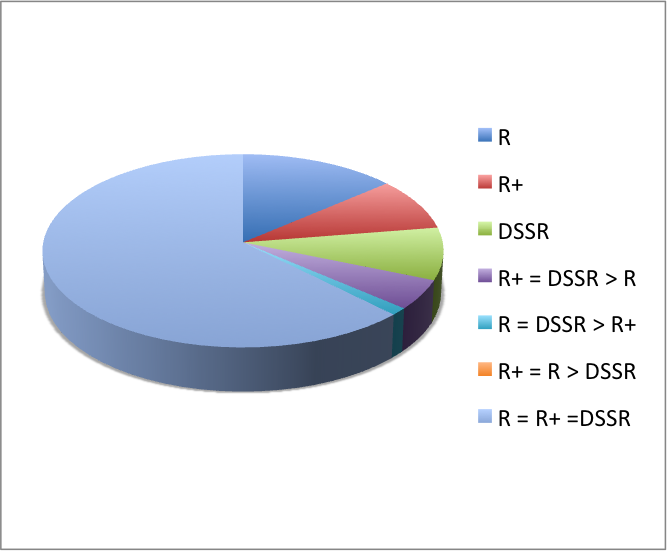
\includegraphics[width=6cm,height=4.5cm]{pie1.png}
\caption{Result Categories.}
\label{fig:pie}
\end{figure}






% // HERE IS THE NEW STRUCTURE
% Present the data with the graphs that Mian generated using Excel.



%%%%%%%%%%%%%%%%%%%%%%%%%%%%%%%%%%%%%%%%%%%%%%%%%%%%%%%%%%%%%%%%%%%%%%%%%%%%%%%%%%%%
%
%  Present each of the 6 categories (best with R, best with R+, best with DSSR, R=R+>DSSR, DSSR=R>R+, and DSSR=R+>R)
%  Add data about the number of classes that are best served with each strategy and which are equivalently in the caption of the figure and in the text.
%
%%%%%%%%%%%%%%%%%%%%%%%%%%%%%%%%%%%%%%%%%%%%%%%%%%%%%%%%%%%%%%%%%%%%%%%%%%%%%%%%%%%

\begin{table}[H]
\caption{Category 1: 50 Experiments where each strategy performed equally well and found same number of faults}
\centering
\begin{tabular}{|l|c|}
\hline\hline
No of Experiments 	& 50  	\\
Mean  			& 12.32  	\\
Median 			& 5 		\\
Standard Deviation 	& 17.73  	\\
Min No of Faults	&  0  		\\
Max No of Faults 	& 96  	\\
\hline
\end{tabular}
\label{table:equal}
\end{table}



%%%%%%%%%%%%%%%%%%%%%%%%%%%%%%%%%%%%%%%%%%%%%%%%%%%%%%



\begin{table}[H]
\caption{Category 2: 11 out of 80 Experiments where Random strategy performed better than DSSR and Random Plus.}
\centering
\begin{tabular}{|l|c|c|c|}
\hline\hline
 				& R			& R+				&  DSSR	\\
\hline
Mean  			&    16.78		&  16.6			&  16.65	\\
Median 			&    17    		&  17				&  17 	\\
Standard Deviation 	&    8.91		&  9.03			&  8.95	\\		
Min No of Faults	&    1			&  1				&  1\\
Max No of Faults 	&    17		&  17				& 17\\
\hline
\end{tabular}
\label{table:Randombetter}
\end{table}

\begin{figure}[ht]
\centering
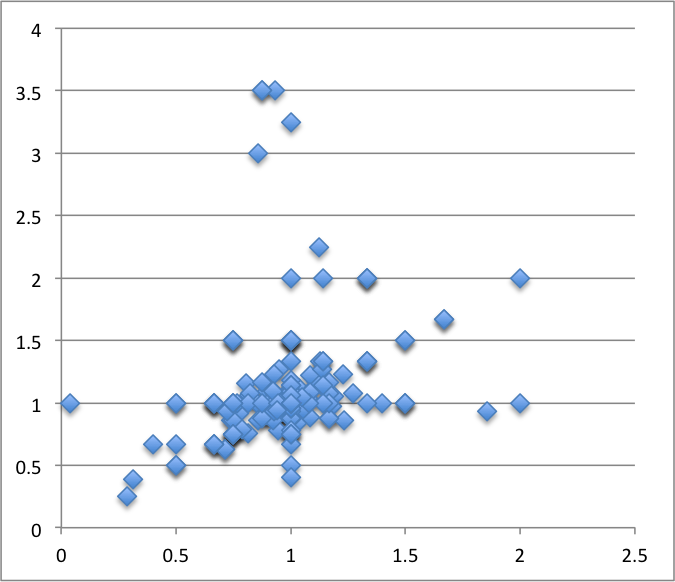
\includegraphics[width=5cm,height=4cm]{Randombetter5.png}
\caption{Random better.}
\label{fig:Randombetter}
\end{figure}



%%%%%%%%%%%%%%%%%%%%%%%%%%%%%%%%%%%%%%%%%%%%%%%%%%%%%%%%%%%%%%%%%%%%%%%%%%%%%%

\begin{table}[H]
\caption{Category 3: 7 out of 80 Experiments where Random Plus strategy performed better than Random and DSSR}
\centering
\begin{tabular}{|l|c|c|c|}
\hline\hline
 				& R			& R+				&  DSSR 	\\
\hline
Mean  			&    26.32		&  26.95			&  26.68\\
Median 			&    7 		&  8	 			&  7.5 \\
Standard Deviation 	&    31.39		&  31.15			&  31.02\\
Min No of Faults	&    1			&  1				&  2\\
Max No of Faults 	&    83		&  83				&  83\\
\hline
\end{tabular}
\label{table:RandomPlusbetter}
\end{table}


\begin{figure}[H]
\centering
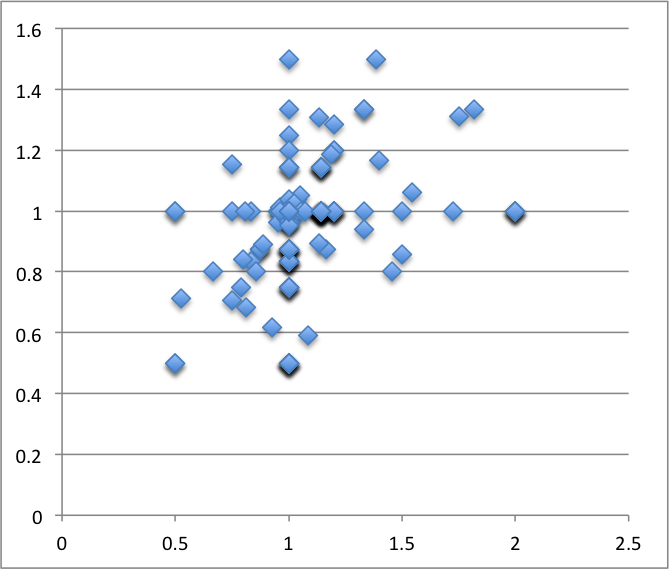
\includegraphics[width=5cm,height=4cm]{RandomPlusbetter5.png}
\caption{Random Plus better.}
\label{fig:RandomPlusbetter}
\end{figure}



%%%%%%%%%%%%%%%%%%%%%%%%%%%%%%%%%%%%%%%%%%%%%%%%%%%%%%

\begin{table}[H]
\caption{Category 4: 7 out of 80 Experiments where DSSR strategy performed better than Random and Random Plus}
\centering
\begin{tabular}{|l|c|c|c|}
\hline\hline
 				& R			& R+ 			& DSSR \\
\hline
Mean  			&    23.44		&  26.32			&  26.36\\
Median 			&    12 		&  12 			&  12 \\
Standard Deviation 	&    15.81		&  14.85			&  14.70\\
Min No of Faults	&    0			&  4				&  4\\
Max No of Faults 	&    45		&  46				&  45\\
\hline
\end{tabular}
\label{table:DSSRbetter}
\end{table}


\begin{figure}[H]
\centering
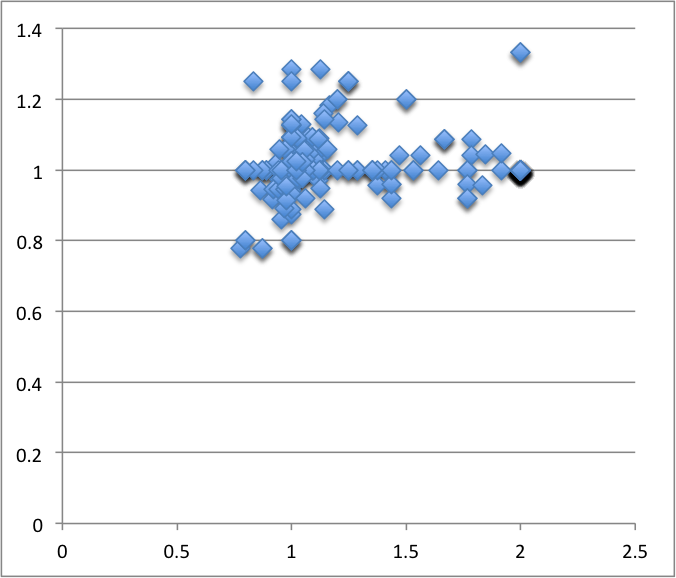
\includegraphics[width=5cm,height=4cm]{DSSRbetter5.png}
\caption{DSSR Better.}
\label{fig:DSSRbetter}
\end{figure}



%%%%%%%%%%%%%%%%%%%%%%%%%%%%%%%%%%%%%%%%%%%%%%%%%%%%%%

\begin{table}[H]
\caption{Category 5: 4 out of 80 Experiments where Random Plus and DSSR performed equally better}
\centering
\begin{tabular}{|l|c|c|}
\hline\hline
 				& R+ = DSSR			&  R \\[1ex]
\hline
Mean  			&    13.76				&  11.18\\
Median 			&    7 				&  5\\
Standard Deviation 	&    15.22				&  11.60\\
Min No of Faults	&    3					&  0\\
Max No of Faults 	&    40				&  31\\
\hline
\end{tabular}
\label{table:DSSRequaltoRandomPlus}
\end{table}

\begin{figure}[ht]
\centering
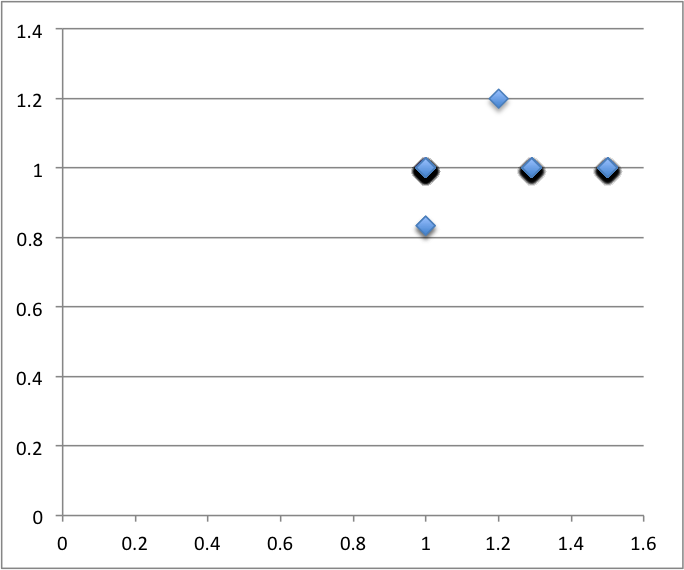
\includegraphics[width=5cm,height=4cm]{DSSRequaltoRandomPlus5.png}
\caption{DSSR equal to RandomPlus.}
\label{fig:DSSRequaltoRandomPlus}
\end{figure}


%%%%%%%%%%%%%%%%%%%%%%%%%%%%%%%%%%%%%%%%%%%%%%%%%%%%%

\begin{table}[H]
\caption{Category 6: 1 out of 80 Experiments where Random and DSSR performed equally better}
\centering
\begin{tabular}{|l|c|c|}
\hline\hline
 				& P = DSSR			&  R+ \\
\hline
Mean  			&    11				&  10.06\\
Median 			&    11 				&  11\\
Standard Deviation 	&    0					&  2.42\\
Min No of Faults	&    11				&  4\\
Max No of Faults 	&    11				&  11\\
\hline
\end{tabular}
\label{table:DSSRequaltoRandom}
\end{table}

\begin{figure}[H]
\centering
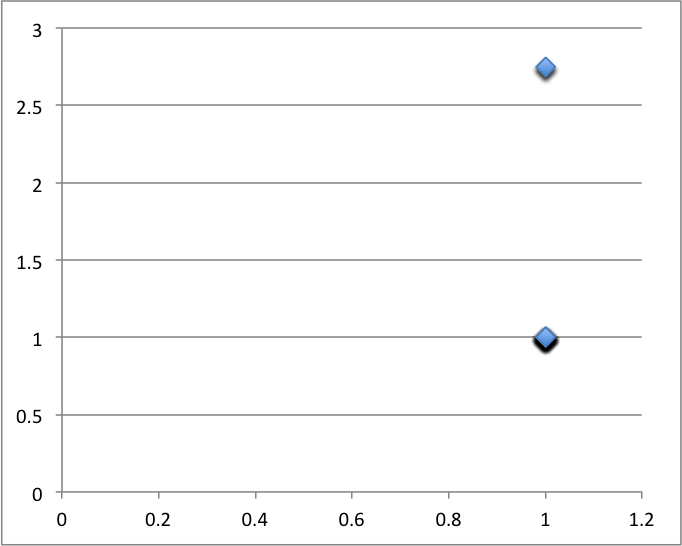
\includegraphics[width=5cm,height=4cm]{DSSRequaltoPureRandom5.png}
\caption{DSSR equal to Pure Random.}
\label{fig:DSSRequaltoRandom}
\end{figure}




\begin{comment}

Conclusions: 
- we show that for roughly 10\% of classes R+ works best, for 10\% DSSR works best, 10\% RT works best
- overall DSSR finds more faults in the same time or number of tests (but this is marginally more than other methods)


Please check if there are more conclusions something with the standard deviation (is it higher, lower etc...) and the minimum as well.

%%%%%%%%%%%%%%%%%%%%%%%%%%%%%%%%%%%%%%%%%%%%





\begin{figure}[H]
\centering
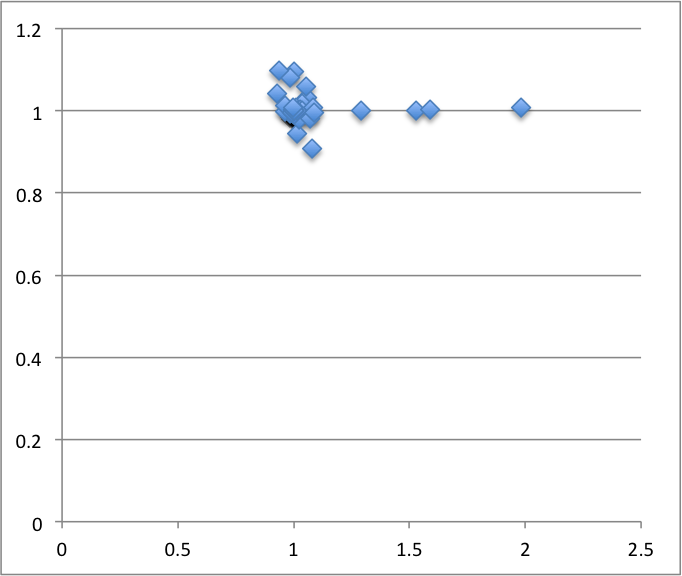
\includegraphics[width=5cm,height=4cm]{combineMean.png}
\caption{Combined Mean.}
\label{fig:Mean}
\end{figure}


\begin{figure}[H]
\centering
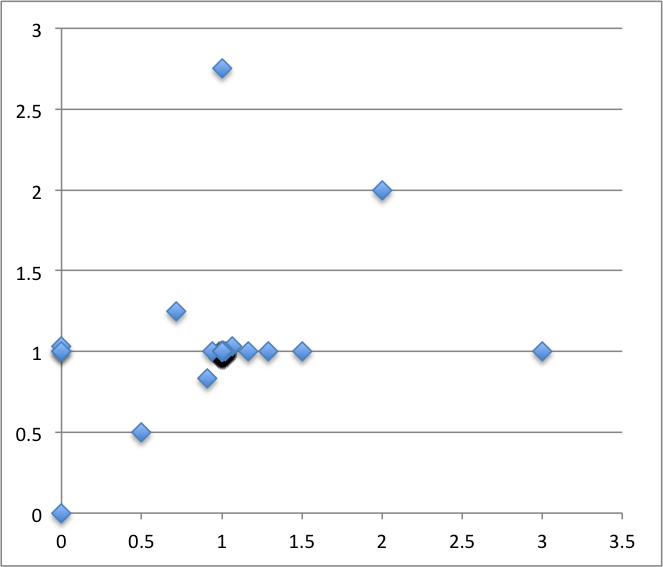
\includegraphics[width=5cm,height=4cm]{combineMin.png}
\caption{Combined Min.}
\label{fig:Min}
\end{figure}


\begin{figure}[H]
\centering
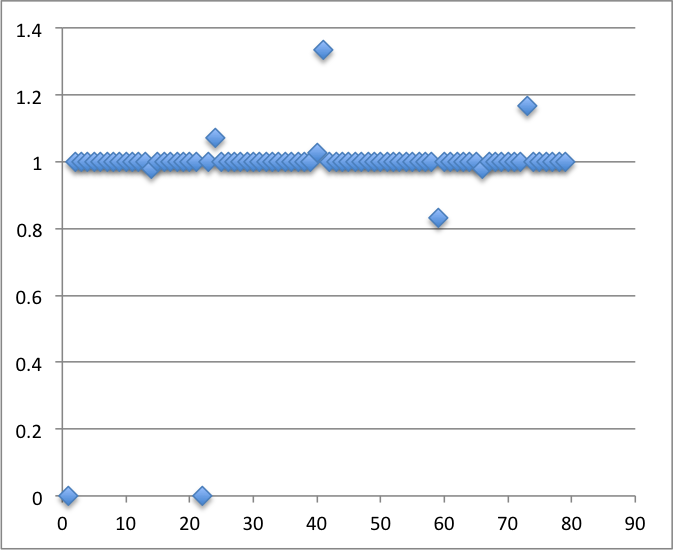
\includegraphics[width=5cm,height=4cm]{combineMax.png}
\caption{Combined Max.}
\label{fig:Max}
\end{figure}


\begin{figure}[H]
\centering
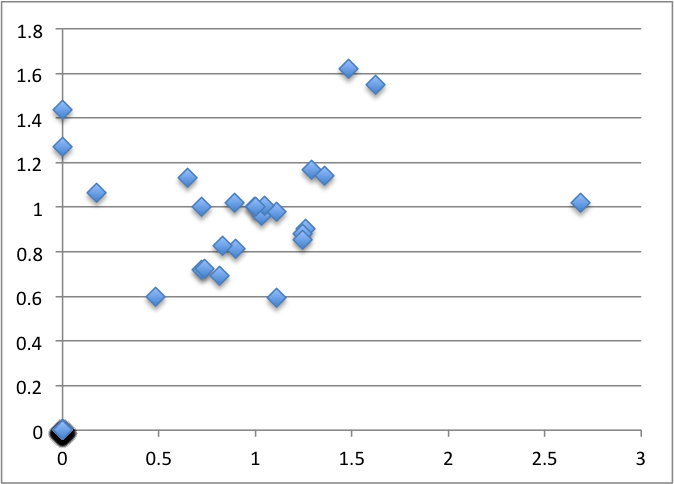
\includegraphics[width=5cm,height=4cm]{combineStdDev.png}
\caption{Combined StdDev.}
\label{fig:StdDev}
\end{figure}



// END NEW STRUCTURE

DSSR has the highest Mean value of finding faults which means that DSSR performs better then random and Random plus. The reason for small improvement instead of 10 and 20\% is described in detail in Discussion section. Similarly the other noticeable improvement is the minimum number of faults DSSR can find is 376 while for random and random plus it is 340 and 344 respectively which means that DSSR strategy always find some of the faults which random and random plus might not. On the other hand DSSR finds maximum 574 faults versus 579 faults of random and random plus but this difference is very small and can be ignored. During the experiments we also found that in some classes like AntClassLoader (Ant project),  Server (Freecs project), BaseFont (itext project) and Util (JsXe project) DSSR strategy found higher number of minimum and maximum faults where as in the same classes random and random plus found 0 or very few faults.  \\

\begin{figure}[ht]
\centering
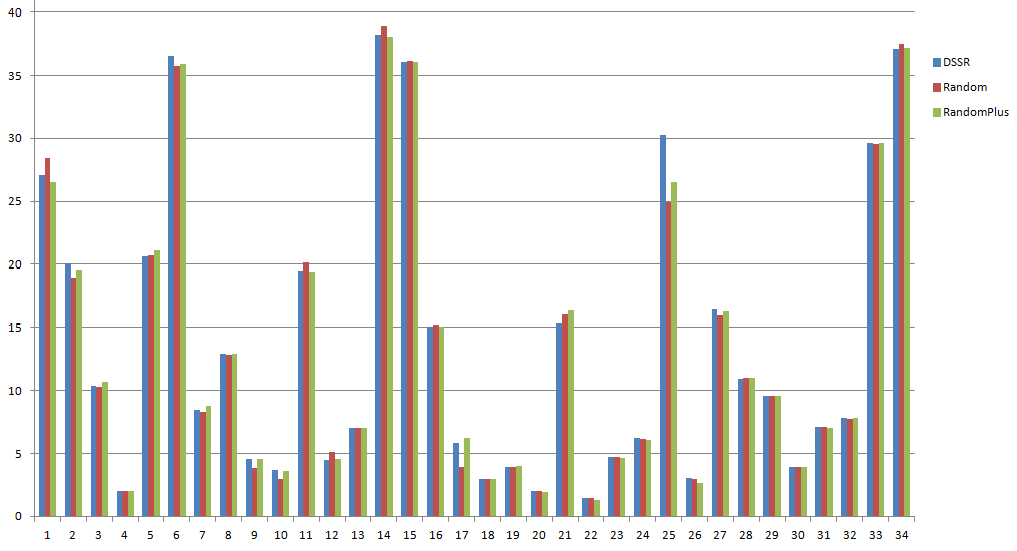
\includegraphics[width=9cm,height=7cm]{newResults.png}
\caption{Test Results of 34 classes from 16 Java projects.}
\label{fig:Result1}
\end{figure}



Figure \ref{fig:Result1} show the results of each experiments using bar chart. From the figure we can see that in few of the cases all the three strategies found equal number of faults while in most cases if not all DSSR performs better than random and random plus strategy.

\end{comment}

%%%%%%%%%%%%%%%%%    DISCUSSION   %%%%%%%%%%%%%%%%%%%%

\section{Discussion}\label{sec:discussion}
\textbf{Performance of DSSR strategy, Random strategy and Random plus strategy in terms of finding faults:} 
Analysis of results revealed that DSSR performs better than random and random plus in programs with block and strip pattern of faults. However, since not all the programs contain faults in the form of block and strip patterns therefore the results do not show a significant performance change. \\
\indent \textbf{Time taken by DSSR strategy, Random strategy and Random plus strategy to execute tests:}
To execute equal number of test cases, DSSR strategy took slightly more execution time than pure random and random plus test strategy. It is not unusual and we were expecting similar behaviour because pure random algorithm selects random input of the required type with minimum calculation and therefore its process is very quick. On the other hand random plus and DSSR strategy performs additional computation when it maintains the list of interesting values and selects the correct type test values from the list when required. The desired process of adding values to the list and selecting the required values from the list consumes extra time which is the main reason that DSSR strategy takes a little extra time. Thus in executing tests random strategy, random plus and DSSR strategy comes first, second and third respectively. \\
\indent \textbf{Effect of test duration in terms of time and number of tests on test results:} 
We found that test duration increases either because of  increase in time or number of test cases which results in improving the performance of DSSR strategy than random and random plus. It is because when test duration or number of tests increases, the list of interesting values also increases and in turn DSSR strategy get enough relevant values in the list of interesting values and can easily pick one from the list instead of selecting it randomly or from static list of random plus.\\
\indent \textbf{Effect of number of faults on results:} 
We also found that DSSR strategy performs better when the number of faults are more in the code. The reason is that when a fault is found in the code, DSSR strategy adds the neighbouring values of the fault finding value to the list of interesting values. Doing this increases the list of interesting values and the strategy is provided with more relevant test data resulting in higher chance of finding faults.\\
\indent \textbf{Can Pure Random and Random Plus Testing perform better than DSSR strategy:}
The experimental results indicated that pure random and random plus testing can perform better than DSSR strategy if the SUT contain point pattern of failures rather than block and strip pattern. It is due to the fact that in such cases faults don't lay in the neighbourhood of found fault and adding neighbouring values of the founded fault dont make any impact on performance therefore the extra computational time becomes a liability.\\
\indent \textbf{DSSR strategy Dependance on Random and Random Plus Testing:}
During the experiments we found that if the fault finding value is not in the list of interesting values then the test is dependant on random testing. In that case DSSR strategy has to wait for random testing to find the first fault and only then DSSR strategy will add its neighbouring values to the list of interesting values.


%%%%%%%%%%%%%%%%%    RW   %%%%%%%%%%%%%%%%%%%%

\section{Related Work}\label{sec:rw}

Random testing is a popular technique with simple algorithm but proven to find subtle faults in complex programs and java libraries \cite{Pacheco2005}, \cite{Csallner2004} and \cite{Claessen2000a}. Its simplicity, ease of implementation and efficiency in generating test cases make it a best choice for test automation \cite{Hamlet1994}. Few of the well known automated tools based on random strategy includes Jartege \cite{Oriat2004}, Eclat \cite{Pacheco2005}, JCrasher \cite{Csallner2004}, AutoTest \cite{Ciupa2007}, \cite{Ciupa2008a} and the latest YETI \cite{Oriol2010}, \cite{Oriol2012}  that is used to conduct this research study.\\

In pursuit of better results and lower overhead many variations of random strategy have been proposed \cite{Chen2010}, \cite{Chen2005}, \cite{Chan2002}, \cite{Chen2004a},\cite{Chen2003}. Adaptive random testing (ART), Quasi-random testing (QRT) and Restricted Random testing (RRT) achieved better results by selecting test inputs random but evenly spread across the input domain. Similarly Mirror ART and ART through dynamic partitioning increased performance by reducing the overhead of ART. One of the main reason behind the better performance of these strategies is that even spread of test input increases the chance of exploring the fault patterns present in the input domain.\\ 

Random plus (R+) strategy \cite{Leitner2007} is a variation of random strategy in which interesting values, beside pure random values, are added to the list of test inputs. These interesting values includes border values \cite{Beizer1990} which has high tendency of finding faults in the given SUT. Results conducted with R+ strategy show significant improvement of pure random strategy. DSSR strategy also rely on R+ strategy in the start until any fault is found where it switches to spot sweeping strategy. \\

It is interesting that numerous efforts have been made to discover the fault patterns \cite{Chen2010}, \cite{Chen2005}, \cite{Chan2002}, \cite{Chen2004a},\cite{Chen2003}, etc. but in our knowledge, none has been published on covering/sweeping all the faults lying in a specific pattern once it has been discovered.\\

A common practice to evaluate performance of newly created or existing strategies is to compare the results obtained (theoretically and empirically) after applying them to similar programs \cite{Gutjahr1999}, \cite{Duran1984}, \cite{Hamlet1990}. We followed similar procedure and evaluated DSSR against R and R+ under constant conditions. \\

Qualitas Corpus \cite{Tempero2010}, a collection of open source java programs maintained for independent empirical research \cite{Oriol2012}, \cite{Tempero2010a}, \cite{Tempero2008}. These projects are carefully selected that spans across the whole set of java applications.

%%%%%%%%%%%%%%%%%    CONCLUSION   %%%%%%%%%%%%%%%%%%%%


\section{Conclusions}\label{sec:conc}
The main goal of the present study was to develop a new random strategy which could find more faults in lower number of test cases and shorter execution time. The experimental findings revealed that DSSR strategy was up to 20\% more effective in finding faults as compared to random strategy and up to 10 \% more effective than random plus strategy. The DSSR strategy not only gave more consistent results but it proved more effective in terms of detecting faults as compared to random and random plus testing.\\
\indent Improvement in performance of DSSR strategy over random strategy was achieved by taking advantage of Random Plus and fault neighbouring values. Random plus incorporated not only border values but it also added values having higher chances of finding faults in the SUT to the list of interesting values.\\
\indent The DSSR strategy is highly effective in case of systems containing block and strip pattern of failure across the input domain.\\
\indent Due to the additional steps of scanning the list of interesting values for better test values and addition of fault finding test value and its neighbour values, the DSSR strategy takes up to 5\% more time to execute equal number of test cases than pure random and random plus. \\
\indent In the current version of DSSR strategy, it might depend on random or random plus strategy for finding the first fault if the fault test value was not in the list of interesting values. Once the first fault is found only then DSSR strategy could make an impact on the performance of test strategy.\\
\indent The limitation of random plus strategy is that it maintains a static list of interesting values which remains the same for each program under test, and can be effective in many cases but not always. The better approach will be to have a dynamic list of interesting values that is automatically updated for every program which can be achieved by adding the program literals and its surrounding values to the list of interesting values prior to starting every new test session.


%%%%%%%%%%%%%%%%%    FUTURE WORK   %%%%%%%%%%%%%%%%%%%%



\section{Future Work}
From the research we came to know that random testing is not very good in generating a test value when the scope of a variable is too narrow as in the following example.  \\
\begingroup
    \fontsize{7pt}{10pt}\selectfont
\noindent
\{ \\*   
\indent if(value == 34.4445) \\*
\indent \{ 10/0 \} \\* 
\} \\*
\endgroup
\indent We also know that if the fault finding value is not in the list than DSSR has to wait for random testing to generate the fault finding value and only after that DSSR strategy will add that value and its surrounding values to the list of interesting values. To decrease the dependancy of DSSR strategy on random and random plus strategy, further work is in progress to add constant literals from the SUT to the list of interesting values in a dynamic fashion. These literals can be obtained either from .java or .class files of the SUT. We are also working to add  neighbouring values of the literals to the list of interesting values. \\
\indent Thus if we have the above example then the value 34.4445 and its surrounding values will be added to the list of interesting values before the test starts and DSSR strategy will no more be dependent on random testing to find the first fault. Finally, it will also be interesting to evaluate the DSSR strategy in terms of coverage because the newly added values are most suitable for test cases and therefore can increase branch coverage. 


%%%%%%%%%%%%%%%%%    ACKNOWDLEGEMENT   %%%%%%%%%%%%%%%%%%%%
\section{Acknowledgment}
The auther would like to acknowldge with thanks the Department of Computer Science, University of York for the financial support extended as Departmental Overseas Research Scholarship (DORS) which enabled him to continue higher studies leading to PhD. We extend our sincere thanks and appreciation to Prof. Richard Page, Head of the Enterprise System's group of the Department of Computer Science for his valuable help and generous support.\\




%%%%%%%%%%%%%%%%%%%%%%%%%%%%%%%%%%%%%%%%%%%%%%%%%%%%%%%%%%%%%%%%%%%%%%%%%%%%%%%%%%%%
%
% Present basic statistical data (max min, mean, std deviation) about each strategy aggregated over all classes.
%
%%%%%%%%%%%%%%%%%%%%%%%%%%%%%%%%%%%%%%%%%%%%%%%%%%%%%%%%%%%%%%%%%%%%%%%%%%%%%%%%%%%



 \begin{table*} [ht] {
  \scriptsize
    \begin{tabular}{|c|l|c|c|c|c|c|c|c|c|c|c|c|c|}
      \hline
      \multirow{2}{*}{S. No}		& \multirow{2}{*}{Class Name}		& \multicolumn{4}{|c|}{R}							&	\multicolumn{4}{|c|}{R+}							&	\multicolumn{4}{|c|}{DSSR}	\\
      \cline{3-14} 
      						&							& mean & max & min & relative std dev				& mean 	& max 	& min 	& relative std dev 		& mean 		& 	max 		&	 min 		& relative std dev \\
             \hline
     
 1						& Routine						& 7	&	7	&	7	& 		0					& 7		&  7		& 7		& 		0			& 7			& 7			& 7			&	0	\\
 2						& Response					& 6	&	6	&	6	& 		0					& 6		&  6		& 6		& 		0			& 6			& 6			& 6			&	0	\\
 3						& Repository					& 31	&	31	&	31	& 		0					& 40		&  40		& 40		& 		0			& 40			& 40			& 40			&	0	\\      
 4						& Rectangle					& 3	&	3	&	3	& 		0					& 3		&  3 		& 3		& 		0			& 3			& 3			& 3			&	0	\\      
 5						& Project						& 64.7&	71	&	60	& 		0.03					& 66.36	&  78		& 62		& 		0.04			& 68.53		& 78			& 64			&	0.04	\\      
 6						& ProjectFactory				& 1	&	1	&	1	& 		0					& 1		&  1		& 1		& 		0			& 1			& 1			& 1			&	0	\\      
 7						& PersistentSet					& 36	&	36	&	36	& 		0					& 36		&  36		& 36		& 		0			& 36			& 36			& 36 			&	0	\\      
 8						& PersistentMap				& 47	&	47	&	47	& 		0					& 47		&  47		& 47		& 		0			& 47			& 47			& 47			&	0	\\      
 9						& PersistentList					& 65	&	65	&	65	& 		0					& 65		&  65		& 65		& 		0			& 65			& 65			& 65			&	0	\\      
 10						& PersistentBag				& 68	&	68	&	68	& 		0					& 68		&  68		& 68		& 		0			& 68			& 68			& 68			&	0	\\      
 11						& Coverage					& 5	&	5	&	5	& 		0					& 5		& 5		& 5		& 		0			& 5			& 5			& 5			&	0	\\      
 12						& NodeSet					& 28.06&	29	&	26	& 		0.02					& 27.86	& 29 		& 26		& 		0.03			& 27.65		& 29			& 26			&	0.03	\\      
 13						& NodeSequence				& 38	&	46	&	30	& 		0.09					& 36.65	& 45 		& 30		& 		0.09			& 36.62		& 44			& 30			&	0.11	\\      
 14						& NameEntry					& 4	&	4	&	4	& 		0					& 4		& 4 		& 4		& 		0			& 4			& 4			& 4			&	0\\      
 15						& Response					& 5	&	5	&	5	& 		0					& 5		& 5 		& 5		& 		0			& 5			& 5			& 5			&	0\\      
 16						& Mat4						& 1	&	1	&	1	& 		0					& 1		&  1		& 1		& 		0			& 1			& 1			& 1			&	0\\      
 17						& List						& 5.27&	6	&	4	& 		0.16					& 5.65	& 6 		& 4		& 		0.09			& 5.34		& 6			& 2			&	0.09\\      
 18						& JmxUtilities					& 7.68&	8	&	6	& 		0.06					& 7.89	& 8 		& 7		& 		0.03			& 7.86		& 8			& 7			&	0.04\\      
 19						& JavaWrapper					& 2	&	2	&	2	& 		0					& 3.93	& 4 		& 3		& 		0.25			& 3.96		& 4			& 3			&	0.18\\      
 20						& ItemSet						& 4	&	4	&	4	& 		0					& 4		& 4 		& 4		& 		0			& 4			& 4			& 4			&	0\\      
 21						& IntStack						& 4	&	4	&	4	& 		0					& 4		& 4 		& 4		& 		0			& 4			& 4			& 4			&	0\\      
 22						& IntHolder					& 1	&	1	&	1	& 		0					& 1		& 1 		& 1		& 		0			& 1			& 1			& 1			&	0\\      
 23						& InstrumentTask				& 1.93&	2	&	1	& 		0.13					& 1.96	& 2 		& 1		& 		0.09			& 2			& 2			& 2			&	0.09\\      
 24						& Image						& 13.89&	18	&	7	& 		0.15					& 12.37	& 14 		& 4		& 		0.20			& 12.89		& 15			& 5			&	0.13\\      
 25						& HttpAuth					& 2	&	2	&	2	& 		0					& 2		& 2 		& 2		& 		0			& 2			& 2			& 2			&	0\\      
 26						& Group						& 11	&	11	&	11	& 		0					& 10.03	& 4 		& 11		& 		0.24			& 11			& 11			& 11			&	0\\      
 27						& Generator					& 17	&	17	&	17	& 		0					& 17		& 17 		& 17		& 		0			& 17			& 17			& 17			&	0\\      
 28						& FPGrowth					& 5	&	5	&	5	& 		0					& 5		&  5		& 5		& 		0			& 5			& 5			& 5			&	0\\      
 29						& Font						& 11.86&	12	&	11	& 		0.02					& 11.86	& 12 		& 11		& 		0.02			& 11.96		& 12			& 11			&	0.01\\      
 30						& FileUtil						& 1	&	1	&	1	& 		0					& 1		& 1 		& 1		& 		0			& 1			& 1			& 1			&	0\\      
 31						& Files						& 3	&	3	&	3	& 		0					& 3		& 3 		& 3		& 		0			& 3			& 3			& 3			&	0\\      
 31						& FileHandler					& 2	&	2	&	2	& 		0					& 2		& 2 		& 2		& 		0			& 2			& 2			& 2			&	0\\      
 33						& Facade						& 3	&	3	&	3	& 		0					& 3		& 3 		& 3		& 		0			& 3			& 3			& 3			&	0\\      
 34						& Entry						& 6	&	6	&	6	& 		0					& 6		& 6 		& 6		& 		0			& 6			& 6			& 6			&	0\\      
 35						& EntryComparator				& 13	&	13	&	13	& 		0					& 13		& 13 		& 13		& 		0			& 13			& 13			& 13			&	0\\      
 36						& EntryDecoder				& 7.93&	9	&	7	& 		0.08					& 8.10	& 9 		& 7		& 		0.09			& 8.13		& 9			& 7			&	0.08\\ 
 37						& Entities						& 3	&	3	&	3	& 		0					& 3		& 3 		& 3		& 		0			& 3			& 3			& 3			&	0\\      
 38						& DOMParser					& 6.75&	7	&	0	& 		0					& 7		& 7 		& 7		& 		0			& 7			& 7			& 7			&	0.18\\      
 39						& DiskIO						& 4	&	4	&	4	& 		0					& 4		& 4 		& 4		& 		0			& 4			& 4			& 4			&	0\\      
 40						& DirectoryScanner				& 32.68&	39	&	0	& 		0.27					& 35.13	& 38 		& 31		& 		0.04			& 35.41		& 39			& 32			&	0.04\\      
 41						& Debug						& 4.62&	6	&	4	& 		0.13					& 4.58	& 6 		& 4		& 		0.12			& 4.86		& 8			& 4			&	0.18\\      
 42						& ColumbaClient				& 3	&	3	&	3	& 		0					& 3		& 3 		& 3		& 		0			& 3			& 3			& 3			&	0\\      
 43						& ClassLoaderLogMan		& 3	&	3	&	3	& 		0					& 3		& 3 		& 3		& 		0			& 3			& 3			& 3			&	0\\      
 44						& CheckAssociator				& 7.06&	8	&	2	& 		0.16					& 6.44	& 9 		& 2		& 		0.33			& 6.96		& 9			& 2			&	0.18\\      
 45						& CatalogManager				& 7	&	7	&	7	& 		0					& 7		& 7 		& 7		& 		0			& 7			& 7			& 7			&	0\\      
 46						& Capabilities					& 1.27&	2	&	1	& 		0.35					& 1.51	& 2 		& 1		& 		0.33			& 1.37		& 2			& 1			&	0.36\\      
 47						& BitSet						& 9	&	9	&	9	& 		0					& 9		& 9 		& 9		& 		0			& 9			& 9			& 9			&	0\\      
 48						& BaseColor					& 14	&	14	&	14	& 		0					& 14		& 14 		& 14		& 		0			& 14			& 14			& 14			&	0\\      
 49						& ArchiveUtil					& 2	&	2	&	2	& 		0					& 2		& 2 		& 2		& 		0			& 2			& 2			& 2			&	0\\      
 50						& Apriori						& 3.10&	4	&	3	& 		0.09					& 3.24	& 4 		& 3		& 		0.13			& 3.17		& 4			& 3			&	0.11\\      
 51						& AntTypeDefinition				& 2.89&	4	&	2	& 		0.27					& 2.75	& 4 		& 2		& 		0.29			& 2.79		& 4			& 2			&	0.23\\      
 52						& AjTypeImpl					& 79.89&	83	&	79	& 		0.01					& 80.06	& 83 		& 79		& 		0.01			& 79.62		& 83			& 79			&	0.01\\      
 53						& AdminCore					& 5	&	5	&	5	& 		0					& 5		& 5 		& 5		& 		0			& 5			& 5			& 5			&	0\\      
 54						& ActionTranslator				& 95.86&	96	&	96	& 		0					& 96		& 96 		& 96		& 		0			& 96			& 96			& 96			&	0\\      
 55						& RubyBigDecimal				& 4 	&	4	&	4	& 		0					& 4		& 4 		& 4		& 		0			& 4			& 4			& 4			&	0\\      
 56						& Scanner					& 3.27&	5	&	2	& 		0.19					& 2.79	& 5 		& 2		& 		0.27			& 3.06		& 5			& 2			&	0.28\\      
 57						& Scene						& 26.10&	27	&	1	& 		0.18					& 25.93	& 27 		& 1		& 		0.18			& 26			& 27			& 1			&	0.18\\      
 58						& SelectionManager				& 3	&	3	&	3	& 		0					& 3		& 3 		& 3		& 		0			& 3			& 3			& 3			&	0\\      
 59						& Server						& 15.51&	21	&	11	& 		0.20					& 16.93	& 12 		& 21		& 		0.16			& 16.93		& 12			& 21			&	0.17\\      
 60						& Sorter						& 1.96&	2	&	1	& 		0.09					& 	3	& 3 		& 3		& 		0			& 3			& 3			& 3			&	0\\      
 61						& Sorting						& 3	&	3	&	3	& 		0					& 	3	& 3 		& 3		& 		0			& 3			& 3			& 3			&	0\\      
 62						& SSL						&13	&	13	&	13	& 		0					& 13		& 13 		& 13		& 		0			& 13			& 13			& 13			&	0\\      
 63						& Statistics					& 14.75&	17	&	12	&	 	0.04					& 23.37	& 25 		& 22		& 		0.03			& 23.44		& 25			& 22			&	0.04\\      
 64						& Status						& 53	&	53	&	53	& 		0					& 53		& 53 		& 53		& 		0			& 53			& 53			& 53			&	0\\      
 65						& Storpwords					& 7.03&	8	&	7	& 		0.02					& 7.68	&  8		& 7		& 		0.06			& 7.65		& 8			& 7			&	0.06\\      
 66						& StringHelper					& 43.41& 45	&	41	& 		0.01					& 44		&  46		& 42		& 		0.02			& 43.55		& 45			& 42			&	0.02\\      
 67						& StringUtils					&19 	&	19	&	19	& 		0					& 19		& 19 		& 19		& 		0			& 19			& 19			& 19			&	0\\      
 68						& TextImpl					& 2 	&	2	&	2	& 		0					& 2		&  2		& 2		& 		0			& 2			& 2			& 2			&	0\\      
 69						& TouchCollector				& 3	&	3	&	3	& 		0					& 3		&  3		& 3		& 		0			& 3			& 3			& 3			&	0\\      
 70						& Trie						& 21.17&	22	&	21	& 		0.01					& 21.10	&  22		& 21		& 		0.01			& 21.03		& 22			& 21			&	0\\      
 71						& URI						& 5 	&	5	&	5	& 		0					& 5		&  5		& 5		& 		0			& 5			& 5			& 5			&	0\\      
 72						& Itextpdf						& 8	&	8	&	8	& 		0					& 8		&  8		& 8		& 		0			& 8			& 8			& 8			&	0\\      
 73						& WebMacro					& 5	&	5	&	5	& 		0					& 5.06	&  6		& 5		& 		0.05			& 5.06		& 7			& 5			&	0.07\\      
 74						& XMLAttributesImpl				& 8	&	8	&	8	& 		0					& 8		&  8		& 8		& 		0			& 8			& 8			& 8			&	0\\      
 75						& XMLChar					& 13	&	13	&	13	& 		0					& 13		&  13		& 13		& 		0			& 13			& 13			& 13			&	0\\      
 76						& XMLEntityManger				& 17.03&	18	&	17	& 		0.01					& 16.95	&  17		& 16		& 		0.01			& 16.96		& 17			& 16			&	0.01\\      
 77						& XMLEntityScanner				& 12	&	12	&	12	& 		0					& 12		&  12		& 12		& 		0			& 12			& 12			& 12			&	0\\      
 78						& XMLErrorReporter				& 5	&	5	&	5	& 		0					& 5		&  5		& 5		& 		0			& 5			& 5			& 5			&	0\\      
 79						& XObject						& 19	&	19	&	19	& 		0					& 19		&  19		& 19		& 		0			& 19			& 19			& 19			&	0\\      
 80						& XString						& 23.86&	24	&	23	& 		0.01					& 23.55	&  24		& 23		& 		0.02			& 23.75		& 24			& 23			&	0.01\\      
    \hline 
    						& Total						&1165.53	& 1181	&    1055	&		5.56					& 1188.73		&	1224	&	1127	&	6.46			& 1192.55		& 1234		& 1126		& 	5.86\\
   \hline
     \end{tabular}
    \label{table:Results}
     }
     \end{table*}




\bibliographystyle{IEEEtran}
\bibliography{bare_conf}

\end{document}


